\chapter{Implementierung}

In diesem Kapitel wird die Implementierung der Ingestion-Schnittstelle besprochen.
In \cref{fig:impl-arch} ist die Systemarchitektur zu sehen.
Diese zeigt alle Komponenten der Schnittstelle und wie diese interagieren.
In den folgenden Abschnitten wird deren Funktionsweise erklärt.
Dabei wird darauf eingegangen, welche Techniken angewendet wurden und warum diese gewählt wurden.
Bei den implementierten Mircoservices wird auch auf entwickelte Algorithmen und Vorgehensweisen eingegangen, mit den bestimmte Aufgaben gelöst werden.
Die Beschreibungen gehen dabei nicht zu sehr ins Detail.
Hier soll eher vermittelt werden, wie ein Problem gelöst wurde, unabhängig von gewählten Rahmenwerken oder Bibliotheken, solange diese nicht notwendig für die Lösung des Problems sind.
Für den API-, Ingestion- und Continuation-Service werden Konfigurationsdateien im YAML-Format\footnote{https://yaml.org/} verwendet.
Über diese werden Verbindungsinformationen und service-übergreifende Parameter konfiguriert.
Am Ende wird auch auf die Bereitstellung eingegangen.
Das heißt wie das fertige System gestartet und verwendet werden kann.


\begin{figure}
    \centering
    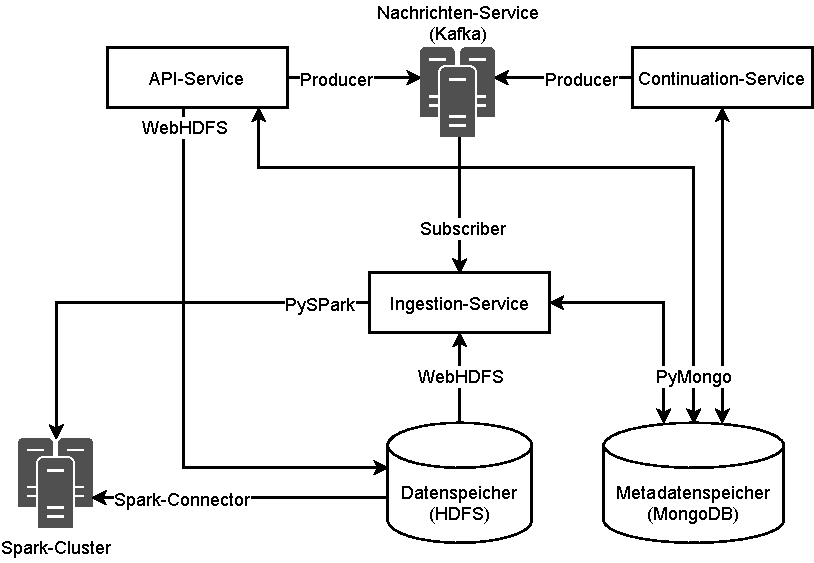
\includegraphics[height=8cm]{Grafiken/Umsetzung-System-Architektur.pdf}
    \caption{Implementierte Systemarchitektur}
    \label{fig:impl-arch}
\end{figure}

\section{Programmiersprache}

Da Apache Spark Implementierungen für Java, Python und Scala bereitstellt, sind das auch die drei Sprachen, auf die die Auswahl begrenzt ist.
Der Prototyp ist in Python geschrieben und da dieser zum API-Service erweitert werden soll, wird Python auch weiter für die Implementierung des API-Service verwendet.
Auch für die Implementierung des Ingestion-Service bietet Python einige Vorteile.

Bei der Verwendung von Java und Scala wird ein fertig kompilierter Job über den Befehl "`spark-submit"' zur Ausführung an Spark gesendet.
Der Spark-Job muss also vor dem Submit bereits kompiliert worden sein.
Daraus folgt, dass es zwei Möglichkeiten gibt, wie der Ingestion-Service damit umgeht.
Zuerst wäre es möglich, dass alle Jobs, die möglicherweise benötigt werden, dem Ingestion-Service bereits kompiliert vorliegen.
Die zweite Möglichkeit wäre, dass die Jobs dynamisch angepasst und immer vor der Ausführung durch den Ingestion-Service kompiliert werden.
Beides würde einen erheblichen Aufwand bei der Entwicklung bedeuten, da entweder ein sehr generischer Job erstellt werden müsste, der alle Ingestion-Fälle abdecken kann, oder es müsste Logik eingebaut werden, die die Quell-Dateien des Jobs bearbeitet und diesen dann kompiliert.

In Python gibt es zusätzlich dazu auch die Möglichkeit, dem Interpreter die Übersetzung zur Laufzeit zu überlassen.
So ist es möglich für jede Anfrage speziell konfigurierte Jobs zu erstellen, die nicht vorher schon kompiliert werden und somit feststehen müssen.
Das senkt die Komplexität bei der Entwicklung der Ingestion \parencite{pyspark-int}.

Auch für die Plugins hat Python einen Vorteil.
Man kann dynamisch Programmcode aus Dateien laden und inspizieren.
So können für jede Ausführung die Plugins einer Datenquelle frisch geladen werden.
Es muss nur dafür gesorgt werden, dass alle Abhängigkeiten erfüllt, also die notwendigen Bibliotheken auf dem Ingestion-Service installiert sind.

Um die Entwicklung einheitlich zu halten, wird auch der Continuation-Service in Python implementiert.
\section{Nachrichten-Service}

Für die Übermittlung von Nachrichten zwischen verschiedenen Anwendungen gibt es sogenannte Message-Broker.
Diese koordinieren als Mittelsmann die Verteilung der Nachrichten an verschiedene Empfänger.
Das hat den Vorteil, dass das Senden und Empfangen asynchron und damit unabhängig voneinander stattfindet \parencite{message-broker}.

Es gibt mittlerweile einige Projekte, die diese Aufgabe auf verschiedene Art lösen.
Hier wird Apache Kafka verwendet, welches im Big Data Bereich weit verbreitet ist, um Datenströme zu verarbeiten.
Daher macht es Sinn, dieses in das Data-Lake-System zu integrieren und darin bereitzustellen.
Um das System dabei nicht unnötig komplex und zu groß werden zu lassen, wird daher auf einen anderen Message-Broker verzichtet.
Außerdem ist die Verteilung der Nachrichten durch Kafka sehr flexibel gestaltbar.

Da Kafka ein Event-Streaming-System ist, wird ab hier nicht mehr von dem Austausch von Nachrichten, sondern von Events gesprochen.
Für diese Events müssen Topics zur Einordnung festgelegt werden.
Die Namen sollten dabei so gewählt werden, dass Kafka auch für andere Datenströme verwendet werden kann, ohne, dass es zu Konflikten kommt.
Daher werden die Topics der internen Kommunikation des Data-Lake-Systems immer mit "`dls\_\_"' als Präfix benannt werden.
Danach folgt der Bereich, den das Event betrifft, hier zum Beispiel "`ingestion"'.
Zu diesem Präfix können noch weitere Informationen hinzugefügt werden.
Für das Ausführen einer Ingestion ist nach diesem Aufbau das Topic "`dls\_\_ingestion\_\_run"'.

Im Ingestion-Service können sehr gut die Gruppen bei Kafka-Konsumenten angewendet werden.
Dazu werden die Konsumenten jedes Ingestion-Service der selben Gruppe hinzugefügt.
So bekommt immer nur ein Ingestion-Service das Event zum Starten einer Ingestion und es muss keine weitere Logik implementiert werden, die sicherstellt, dass nicht mehrere Ingestion-Services eine Ingestion zur gleichen Quelle starten.
Das macht die Skalierung und Verteilung der Ingestion-Services sehr einfach.
\section{Metadaten-Management-System}

Da das Metadatenmodell einer Datenquelle eine verschachtelte Struktur hat, bietet sich hier als einfachste Lösung die Verwendung einer dokumenten-orientierten NoSQL-Datenbank an.
Das hat den Vorteil, dass die Sammlungen von Revisionen und IngestionEvents direkt in den Objekten der DatasourceDefinition abgelegt werden können.
In relationalen Datenbank-Systemen müsste man für jedes Modell eine eigene Tabelle erstellen und die Verknüpfungen über mehrere Abfragen zusammenführen.
Bei jeder Abfrage einer Datenquelle werden die verknüpften Einträge der IngestionEvents oder Revisionen gebraucht, was somit zu einem größeren Aufwand führt.
Außerdem gibt es viele Anfragen auf die Datenquellen, da diese nicht zwischen den Mircoservices ausgetauscht werden und so nicht im Speicher vom Service verwaltet werden können.
Daher ist es effizienter die relevanten Daten direkt mit einer Abfrage laden zu können.
Hier kann auch wieder eine Komponente aus dem Prototyp übernommen werden.
Deswegen kommt MongoDB\footnote{https://www.mongodb.com/} als Datenbank-System zum Einsatz.

\section{Datenspeicher}

Für das Speichern von Daten mit einer Versionierung ist Delta Lake eine gut gepflegte und in Spark integrierte Lösung.
Da im Delta Lake Datensätze immer versioniert werden, muss auch ein Speicher für unversionierte Daten bereitgestellt werden.
Für strukturierte und semistrukturierte Daten kommt das Parquet-Format zum Einsatz.
Unstrukturierte Daten werden im ursprünglichen Format im HDFS abgelegt.

Als Speicher wird das HDFS verwendet.
In diesem können sowohl die Delta Tabellen als auch andere Parquet-, Quell- und Plugin-Dateien abgelegt werden.
Alle Microservices haben über die WebHDFS-Schnittstelle Zugriff auf die Daten.
Im HDFS wird eine Verzeichnisstruktur (\cref{fig:hdfs-folder}) für alle Daten des Data Lake angelegt.
Diese geht von dem Ordner "`datalake"' aus, der im Root-Verzeichnis des HDFS angelegt wird.
In diesem Ordner werden die Unterordner
\begin{itemize}
    \item "`sources"' für Quell-Dateien,
    \item "`plugins"' für Plugin-Dateien und
    \item "`data"' für die Ablage von geladenen Daten erstellt.
\end{itemize}

In den Ordnern "`sources"' und "`plugins"' werden dann für jede Datenquelle Ordner mit deren Id angelegt, in denen die hochgeladenen Dateien abgelegt werden.

Für die geladenen Daten werden die Ordner \begin{itemize}
    \item "`structured"' für semi-/strukturierte Daten ohne Versionierung,
    \item "`unstructured"' für unstrukturierte Daten und
    \item "`delta"' für semi-/strukturierte Daten mit Versionierung
\end{itemize}
innerhalb des Ordners "`data"' angelegt.
Diese unterteilen sich dann ebenfalls wieder in Ordner für jede Datenquelle mit der Id als Name.

\begin{figure}
    \centering
    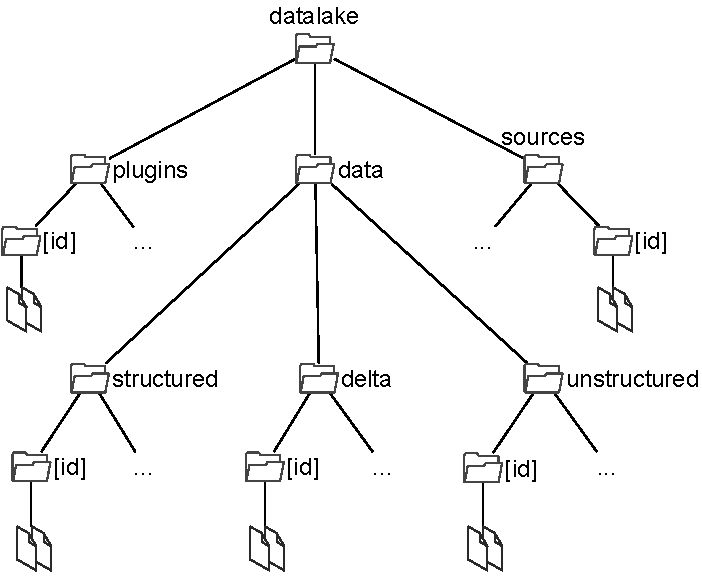
\includegraphics[width=.6\textwidth]{Grafiken/Umsetzung-Verzeichnisse.pdf}
    \caption{HDFS Verzeichnisstruktur}
    \label{fig:hdfs-folder}
\end{figure}
\section{API-Service}

Bei HTTP-Anfragen können Inhalte in der Anfrage als verschiedene Typen übergeben werden.
Hier wird der Typ \verb|mutltipart/forma-data| verwendet.
Bei diesem Typ können sowohl Text als auch Dateien übertragen werden.
Jeder Text oder jede Datei werden dabei als Wert betrachtet und müssen einen Schlüssel vergeben bekommen.
Das heißt, dass alle Informationen als Schlüssel-Wert-Paar an den API-Service gesendet werden.
Die Schlüssel, die verwendet werden sollen, werden wie folgt vergeben.
Die DatasourceDefinition bekommt den Schlüssel "`datasource-definition"'.
Der Wert dahinter kann entweder eine JSON-Datei oder ein JSON-Text sein.
Die Schlüssel der hochgeladenen Dateien sind frei wählbar.

Die DatasourceDefinition besteht zu Teilen aus Feldern, die automatisch durch die Services gefüllt werden.
Daher wird ein weiteres Datenmodell für die Eingabe von Informationen bei der REST-API benötigt.
Dafür wird die DatasourceDefinitionInput (\cref{fig:datasource-definition-input}) verwendet.
In diesem Modell befinden sich alle Felder, die durch den Benutzer befüllt werden können.
Aus den Daten dieses Modells erstellt der API-Service dann die Revisionen für die DatasourceDefinition.

\begin{figure}
    \centering
    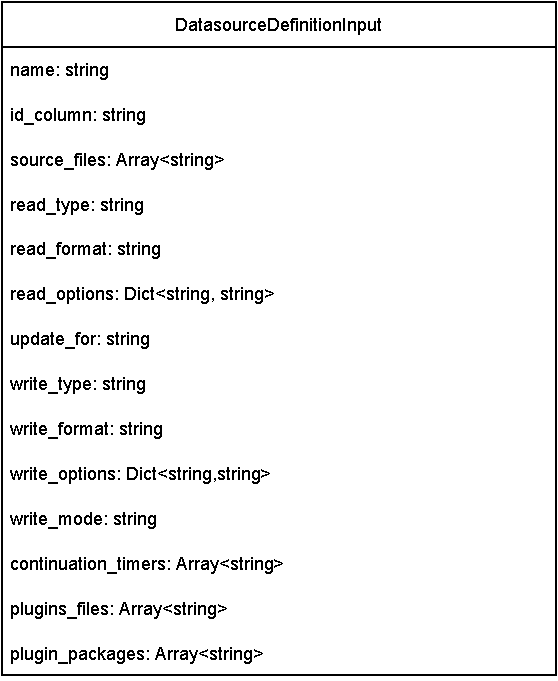
\includegraphics[width=.65\textwidth]{Grafiken/Umsetzung-Definition-Input.pdf}
    \caption{Felder Datenquellen-Eingabe}
    \label{fig:datasource-definition-input}
\end{figure}

\subsection{Hochladen von Dateien}

Für jede Datenquelle können Quell- oder Plugin-Dateien hochgeladen werden.
Um eine hochgeladene Datei in der Datenquelle auch zu verwenden, muss der Schlüssel, unter dem die Datei hochgeladen wird, in der entsprechenden Liste entweder unter "`source\_files"' oder unter "`plugin\_files"' hinzugefügt werden.
Alternativ können auch die Namen unter denen bereits Dateien für die Datenquelle gespeichert wurden in die Listen eingefügt werden.

Bei der Verarbeitung der Eingabe prüft der API-Service für jeden Eintrag der Listen, ob eine Datei mit diesem Schlüssel hochgeladen wurde.
Ist das der Fall, wird die entsprechende Datei in das HDFS hochgeladen.
Der Name, unter dem die Datei gespeichert wird, setzt sich aus der Nummer der Revision, dem vergebenen Schlüssel und der Endung der Datei zusammen.
Lädt man also eine bei der ersten Erstellung einer DatasourceDefinition eine Datei "`data.json"' mit den Schlüssel "`file"' hoch, wird diese als "`r000\_file.json"' im "`sources"'-Ordner der DarasourceDefinition gespeichert.
Analog werden Plugin-Dateien genauso behandelt.

Wenn keine Datei in der Anfrage gefunden wurde, wird geschaut, ob im HDFS eine Datei mit dem Namen existiert.
Wird eine Datei gefunden, wird der Name an die neue Revision angehangen.
Es ist wichtig zu beachten, dass alle Dateien der alten Revision, die nicht explizit in einer der Listen angegeben werden, nicht in der neuen Revision verwendet werden.
Sie bleiben jedoch gespeichert und können später wieder hinzugefügt werden.
Da die Dateien nach den Datenquellen aufgeteilt sind, ist es aktuell nicht möglich Plugins oder Quell-Dateien in anderen Datenquellen wieder zu verwenden.
Hier müsste man die Datei für jede Datenquelle hochladen.

\section{Continuation-Service}

Der Continuation-Service führt durchgehend eine Schleife zum Überprüfen der Datenquellen aus.
Alle für die Schleife benötigten Informationen werden aus dem Metadatenspeicher geladen.
Bei der Prüfung wird immer der Status des aktuellsten IngestionEvent betrachtet.
Je nach Datenquelle wird dann entschieden, ob eine Ingestion gestartet werden soll.
Die Logik der Schleife besteht aus drei Teilen, wovon zwei die Datenquellen prüfen und einer die Zeit steuert, nachdem die Schleife erneut ausgeführt wird (\cref{algo:ci-loop}).
Das soll nur maximal jede Minute geschehen, da auch keine schnellere Ausführung über die Timer definiert werden kann.

Im ersten Teil werden alle Datenquellen einer Datenstrom-Ingestion kontrolliert.
Für diese wird eine neue Ingestion gestartet, wenn der Status "`FINISHED"' ist.
Der Status "`STOPPED"' bedeutet, dass die Ausführung mit Absicht beendet wurde und manuell gestartet werden muss.

Der zweite Teil überprüft alle Datenquellen, bei denen ein oder mehrere Timer gesetzt wurden.
Wenn der Status des letzten IngestionEvents nicht "`STOPPED"' oder "`FINISHED"' ist, wird die Überprüfung dieser Quelle abgebrochen.
Ansonsten wird jeder Timer mit dem aktuellen Zeitpunkt verglichen.
Hier wird die Methode $is\_now$ verwendet.
Sie wird durch eine Python-Bibliothek bereitgestellt und prüft, ob ein Cron-Timer, die auch für die kontinuierliche Ingestion eingesetzt werden, zum aktuellen Zeitpunkt zutrifft.
Trifft der Timer zu, wird eine Ingestion für die Datenquelle gestartet und sofort die nächste Datenquelle überprüft.

Der dritte Teil kontrolliert die Ausführungshäufigkeit.
Dazu wird am Anfang der Schleife der Startzeitpunkt gespeichert.
Nachdem alle Überprüfungen beendet wurden, wird auch der Endzeitpunkt gespeichert.
Wenn die Differenz der beiden geringer ist als eine Minute, wird die Schleife für die Dauer der Differenz angehalten.
Damit ist sichergestellt, dass sie nicht häufiger als einmal pro Minute ausgeführt wird.

\begin{algorithm}
    \caption{Continuation loop}
    \label{algo:ci-loop}

    $loopStart \gets$ current\_time() \;

    $streams \gets$ all\_datasource\_definition\_of\_type\_stream() \;
    \ForAll {$definition$ in $streams$} {
        $event \gets definition.last\_ingestion$ \;
        \If {$event.state$ is FINISHED} {
            publish\_run\_event\_for($definition.id$) \;
        }
    }

    $timed \gets$ all\_datasource\_definitions\_with\_timers() \;
    \ForAll {$definition$ in $timed$} {
        $event \gets definition.last\_ingestion$ \;
        $timers \gets definition.revision.continuation\_timers$  \;
        \If {$event.state$ is STOPPED or FINISHED} {
            \ForAll {$timer$ in $timers$} {
                \If {is\_now($timer$)} {
                    publish\_run\_event\_for($definition.id$) \;
                    \textbf{break}
                }
            }
        }
    }

    $loopEnd \gets$ current\_time() \;
    $loopDuration \gets loopEnd - loopStart$ \;
    \If {$loopDuration < 60$} {
        sleep($60 - loopDuration$) \;
    }

\end{algorithm}


\section{Ingestion-Service}

Wie in \cref{sec:entw-ingestion} beschrieben, wird für eine Ingestion ein Prozess gestartet.
Zum Starten einer Ingestion wird das Topic "`dls\_\_ingestion\_\_run"' verwendet.
In \cref{sec:ingestion-run} wird der detailliere Ablauf mit den verschiedenen Wegen für Read- und SaveTypes beschrieben.
Vorher werden die benötigten Grundlagen zur Ausführung erläutert.

\subsection{Berechnen und Speichern der Änderungsdaten}
Um Änderungen in eine Delta-Tabelle zu übernehmen, müssen die Änderungsdaten in einem Format sein, dass Aufschluss darüber gibt, welche Daten hinzugefügt, welche geändert und welche gelöscht worden sind.
Das hier verwendete Format muss genau dem Schema der Originaldaten entsprechen.
Zusätzlich soll eine Spalte oder ein Feld auf der obersten Ebene mit dem Namen "`cd\_deleted"' vorhanden sein.
Darin ist ein Boolean-Wert enthalten, der aussagt, ob der Eintrag aus den Daten gelöscht wurde oder nicht.
Der Datensatz mit den Änderungsdaten darf außerdem nur geänderte Daten enthalten.
Aus diesem Format können, wie später gezeigt, die drei Operationen abgeleitet werden.

Um nicht auf ein externes Change-Data-Capture-System angewiesen zu sein, gibt es eine interne Lösung, die auf alle (semi-)strukturierten Daten angewendet werden kann.
Dazu eignet sich der in \cref{sec:snaps} genannte snapshot-basierte Ansatz.
Dieser ist zwar langsamer als alle anderen, aber auch als einziger unabhängig von der Datenquellen und innerhalb des Data-Lake-Systems anwendbar.

\textcite{snapshot_algos} haben einen Algorithmus vorgestellt, der diese Aufgabe mit der Hilfe von Join-Operationen löst.
Für den Vergleich werden für jeden Eintrag eindeutige Schlüssel benötigt.
Das Feld "`id\_column"' in der DatasourceDefintion enthält den Namen der Spalte oder des Feldes, das als Schlüssel fungieren soll.
Es können auch verschachtelte Felder verwendet werden.
Der Schlüssel kann aber nicht aus mehreren Feldern zusammengesetzt werden.
Die Namen der Felder in den einzelnen Ebenen müssen dafür mit einem "`."' getrennt werden.
Beispielsweise "`user.id"' für: \begin{verbatim}
    {
        user: { 
            id: x 
        }
        ...
    }
\end{verbatim}

Join-Algorithmen sind in der Informatik bereits vielfach besprochen worden.
Wenn man die Einträge beider Snapshots über ihren Schlüssel verknüpft, kann man so durch einen Vergleich der Ergebnisse alle geänderten Einträge finden.
In einem Full-Outer-Join sind zusätzlich alle Einträge vorhanden, die nur in einem der beiden Einträge vorhanden sind.
Die restlich Felder bekommen einen Null-Wert.
Je nachdem auf welcher Seite die Null-Werte stehen, handelt es sich um eine Einfügung oder Löschung.
Da durch SparkSQL eine gute Unterstützung für Join-Operationen gegeben ist, ist dieser Ansatz auch gut für den Einsatz im Data Lake geeignet.
Dieses Vorgehen funktioniert sowohl für relationale als auch semistrukturierte Daten.
Bei dem Vergleich von semistrukturierten Daten wird jedoch nur die oberste Ebene als Spalte betrachtet.
Alle darunter verschachtelten Objekte werden als Werte dieser Spalten betrachtet.

Der \cref{algo:delta-calc} zum Vergleich von DataFrames orientiert sich an diesem Vorgehen.
Als Eingabe werden ein linkes DataFrame, mit dem aktuellen internen Stand, eine rechtes DataFrame, mit den neuen Daten und der Name des Schlüssels benötigt.
Um den Vergleich der Zeilen später einfacher zu machen, wird zuerst für jede Zeile der zu vergleichenden Datensätze ein Hashwert über alle Spalten berechnet.
Außerdem wird eine weitere Spalte mit dem Namen "`\char`~ id"' hinzugefügt, die den Wert des Schlüssels zugewiesen bekommt.
Da wie bereits erwähnt bei semistrukturierten Daten nur die oberste Ebene als Spalten betrachtet wird, ist es so erst möglich  Einträge über verschachtelte Schlüssel zu verknüpfen.
Danach wird ein Full-Outer-Join über den Daten ausgeführt.
Im nächsten Schritt werden alle Zeilen, in denen die Hashwerte gleich sind aus dem Datensatz entfernt, da diese keine Relevanz für die Änderungsdaten haben.
Zu den gefilterten Daten wird nun die Spalte "`cd\_deleted"' hinzugefügt.
Ist in den alten Daten eine Zeile vorhanden und in den neuen nicht mehr, so ist der Hashwert auf der rechten Seite $Null$.
In diesem Fall bekommt die Spalte "`cd\_deleted"' den Wert $true$ für alle anderen ist der Wert $false$.
Da das Ergebnis der Join-Operation alle Spalten doppelt enthält, einmal von links und einmal von rechts, müssen diese noch zusammengeführt werden.
Dazu können immer, außer bei dem Schlüssel, die Werte der rechten Seite genommen werden, da diese die neuen Werte enthält.
Der Wert für den Schlüssel wird auch von der rechten Seite übernommen, es sei denn dieser ist $Null$ (bei gelöschten Zeilen), dann muss der linke Wert verwendet werden, da der Schlüssel nicht $Null$ sein darf.
Zum Schluss müssen die zusätzlich für den Vergleich hinzugefügten Spalten wieder entfernt werden.
Das Ergebnis ist ein DataFrame mit allen Änderungen.
Es hat das gleiche Schema wie die Ursprungsdaten, aber mit der zusätzlichen Spalte "`cd\_deleted"', die Auskunft darüber gibt, ob ein Datensatz gelöscht wurde.

\begin{algorithm}
    \caption{Deltaberechnung}
    \label{algo:delta-calc}
    \textbf{Input:} $left$: DataFrame, $right$: DataFrame, $id\_column$: String  \\
    \textbf{Output:} $change\_data$: DataFrame \\

    \ForAll{$df$ \textbf{in} $[left, right]$}{
        $df$.add\_column($name$: "`hash"', $value$: $df$.hash\_over\_all\_rows())\;
        $df$.add\_column($name$: "`\char`~ id"', $value$: $df$.get\_value($id\_column$))\;
    }

    $change\_data \gets$ $left$.join($right$, $type$: full-outer, $column$: "`\char`~ id"')\;
    $change\_data$.remove\_all\_row($condition$: $left.hash$ equals $right.hash$)\;
    $change\_data$.add\_column($name$: "`cd\_deleted"', $value$: $false$)\;

    \ForAll{$row$ \textbf{in} $change\_data.rows$}{
        \If{$row.right.hash$ \textbf{is} $Null$}{
            $row.cd\_deleted \gets true$\;
        }
    }

    \ForAll{$column$ \textbf{in} $left.columns$}{
        \eIf{$column$ \textbf{is} $id\_column$}{
            \ForAll{$row$ \textbf{in} $change\_data.rows$}{
                \eIf{$row.right.hash$ \textbf{is} $Null$}{
                    $row.id\_column \gets row.left.id\_column$\;
                } {
                    $row.id\_column \gets row.right.id\_column$\;
                }
            }
        }{
            \ForAll{$row$ \textbf{in} $change\_data.rows$}{
                $row.column \gets row.right.column$\;
            }
        }
        $change\_data$.remove\_column($right.column$)\;
        $change\_data$.remove\_column($left.column$)\;
    }
    $change\_data$.remove\_column("`\char`~ id"')\;
    $change\_data$.remove\_column("`hash"')\;

\end{algorithm}

Das Einpflegen der Änderungen unterscheidet sich nach dem gewählten Speicherziel.
Für Delta-Tabellen wird die Delta Lake API verwendet.
Dazu werden die Änderungsdaten mit den aktuellen Daten über den Schlüssel zusammengeführt.
Dabei können verschiedene Fälle definiert werden.
Wenn die Ids einer Zeile gleich sind und die Spalte "`cd\_deleted"' $true$ enthält, wird die Zeile aus den Daten gelöscht, ansonsten wird der Datensatz aktualisiert.
Wenn die Ids nicht übereinstimmen und die Spalte "`cd\_deleted"' $false$ ist, wird der Datensatz als neue Zeile eingefügt.

Für Parquet-Dateien werden die Änderungsdaten über Spark mit den Bestandsdaten zusammengeführt.
Beide Datensätze werden über einen Full-Outer-Join verknüpft.
Danach werden alle Zeilen, in denen das Feld "`cd\_deleted"' den Wert $true$ enthält, gelöscht.
Ähnlich zu der Deltaberechnung werden die übrigen Daten wieder auf das Originalschema gebracht.
Dabei werden für alle Zeilen, bei denen entweder kein Eintrag aus den Bestandsdaten existiert oder die Änderungsdaten sich von ihnen unterscheiden, die Werte der Änderungsdaten übernommen.
In den anderen Zeilen werden die Bestandsdaten beibehalten.

\subsection{Plugin-Management}

Da Python verwendet wird, kann nicht, wie zum Beispiel in Java, ein Interface definiert werden, dass ein Plugin implementieren muss.
Es ist aber möglich die Namen, Parameter und Rückgabetyp einer Methode zu überprüfen.
Mit diesem Ansatz können Methoden aus den hochgeladen Plugin-Dateien validiert werden.
Für die Ingestion werden diese zwei Methoden definiert: \begin{enumerate}
    \item Load-Methode: \begin{verbatim}
        Name: "load"
        Rückgabetyp: DataFrame
        Parameter:
            - Name: "spark"
              Typ: SparkSession
    \end{verbatim}
    \item After-Load-Methode: \begin{verbatim}
        Name: "after_load"
        Rückgabetyp: DataFrame
        Parameter:
            - Name: "dataframe"
              Typ: DataFrame
    \end{verbatim}
\end{enumerate}

Für jede Ingestion wird auf dem Speichersystem des Mircoservices ein temporärer Ordner angelegt, in den die Plugin-Dateien abgelegt und deren Abhängigkeiten installiert werden.
Nach der Installation wird noch eine Datei angelegt, die für alle Pakete die Versionsnummern enthält.
Das dient dazu, bei einer erneuten Ausführung auf dem Service nicht alle Pakete neu installieren zu müssen, sondern nur die mit einer geänderten Versionsnummer.
Das beschleunigt die Ausführung der Ingestion.
Zum Schluss wird der Ordner, mit den installierten Paketen, zum Python-Pfad hinzugefügt.
Damit wird dieser während der Ausführung manipuliert und die Pakete sind verfügbar.
Da jede Ingestion in einem eigenen Prozess ausgeführt wird, beeinflussen die Änderungen an dem Python-Pfad den Ingestion-Service oder andere Prozesse nicht.

Im zweiten Schritt wird jede Plugin-Datei als Python-Modul geladen.
Jedes Modul enthält dann die in der Plugin-Datei definierten Methoden.
Diese Methoden können mit den Definitionen verglichen werden.
Dazu wird der \cref{algo:check-method} verwendet.
Diesem werden das geladene Modul, ein Name der Methode, ein optionaler Rückgabetyp der Methode und eine Liste von Parametern, bei denen Name und Typ definiert sind.
Zur Überprüfung können alle Methoden in dem Modul auf ihren Namen geprüft werden.
Wenn eine Methode gefunden wurde, wird eine Signatur erzeugt und mit der übergebenen Definition verglichen.
Das Ergebnis sagt dann, ob diese Methode ein Plugin ist oder nicht.

Jedes geladene Modul wird auf die Load- oder AfterLoad-Methoden geprüft.
Eine gefundene Load-Methode überschreibt immer die vorher gefundene, da jede Ingestion nur einen Weg zum Laden der Daten haben darf.
Die After-Load-Methoden dagegen werden in einer Liste gespeichert.
Es kann jedoch immer nur eine After-Load-Methode pro Plugin-Datei geben.
Diese können dann auch hintereinander ausgeführt werden, um auf einem DataFrame mehrere Modifikationen auszuführen.
Alle gefunden Methoden werden in einem Plugin-Manager gespeichert, um während der Ingestion aufgerufen werden zu können.
Die Reihenfolge der Ausführung entspricht der Reihenfolge, wie die Plugin-Dateien bei der Erstellung in der Liste angegeben wurden.

\begin{algorithm}
    \caption{Pluginmethode überprüfen}
    \label{algo:check-method}

    \textbf{Input:} $plugin$: Python-Modul, $name$: String, $return\_type$: Typ, $parameters$: Liste \\
    \textbf{Output:} $matches$: Boolean \\

    \If{$plugin$ \textbf{has no} method $name$}{
        \Return{false}
    }

    $signature \gets$ signature of mehtod $name$

    \If{$signature.return\_type$ \textbf{is not} $return\_type$}{
        \Return{false}
    }

    \ForAll{$param$ \textbf{in} $parameters$}{
        \If{$signature$ \textbf{has no} parameter $param.name$}{
            \Return{false}
        }
        \If{$signature.parameter.type$ \textbf{is not} $parameter.type$}{
            \Return{false}
        }
    }
    \Return{true}

\end{algorithm}

\subsection{Ausführung der Ingestion}
\label{sec:ingestion-run}
Die Ausführung startet mit der Initialisierung, welche die für die Ingestion benötigte Daten lädt.
Das ist zum Beispiel die DatasourceDefinition zu der Id aus den Events.
Danach wird entschieden, ob eine Ingestion über Spark notwendig ist.
Hier spielt der Lesetyp eine große Rolle.
Bei der Ingestion von unstrukturierten Daten wird Spark nicht benötigt.
Hier können die Dateien, über die WebHDFS-Schnittstelle direkt im HDFS verschoben werden.
Für alle anderen Typen wird im nächsten Schritt die Ingestion vorbereitet.
Es werden die Plugins aus dem HDFS geladen und eine SparkSession erstellt.
Das Laden der Daten in ein DataFrame geschieht anschließend entweder über ein Plugin in oder das Standardvorgehen.
Falls auch After-Load-Plugins vorhanden sind, werden diese ausgeführt.
Für die geladenen Daten wird dann entschieden, ob es sich um Änderungsdaten handelt oder welche berechnet werden müssen.
Je nach Schreib-Typ werden dann die Daten beziehungsweise Änderungsdaten gespeichert.
Für Datenströme wird am Ende noch ein Hintergrund Task gestartet, der auf Kafka Events zum Stoppen dieser Ingestion wartet.
Hierfür wird das Topic "`dls\_\_ingestion\_\_stop\_ingestion"' mit der Id als Wert verwendet.
Wenn die Ingestion beendet wurde, wird zum Schluss die SparkSession gestoppt.

\begin{figure}
    \centering
    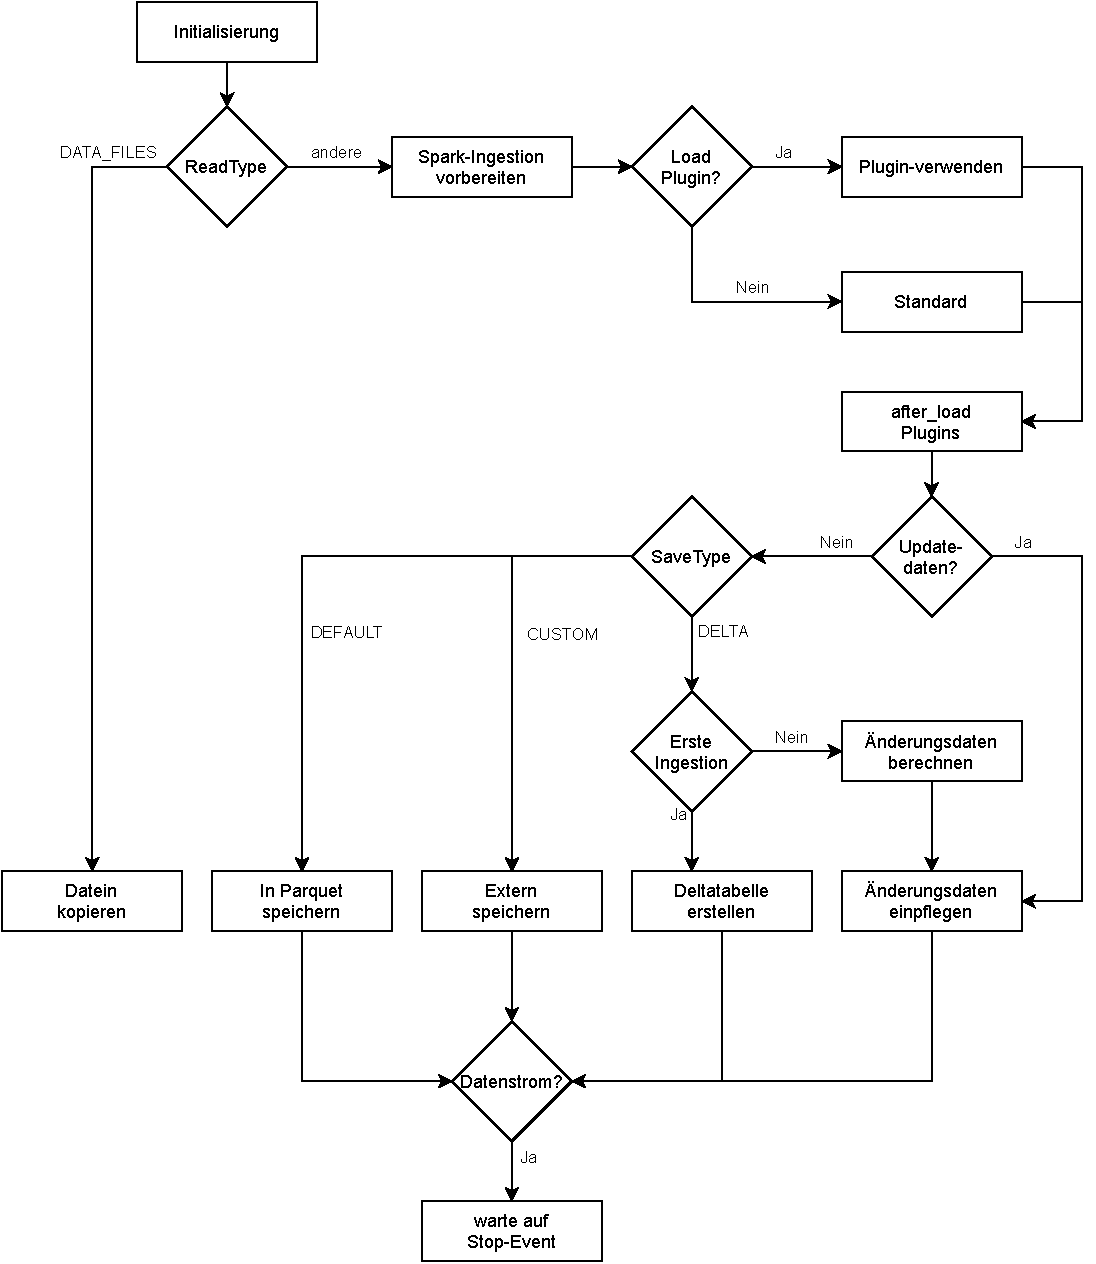
\includegraphics[width=\textwidth]{Grafiken/Umsetzung-Ingestion-Ablauf.pdf}
    \caption{Ablauf einer Ingestion}
    \label{fig:umsetz-ingestion-ablauf}
\end{figure}
\section{Bereitstellung}

Bei der Bereitstellung des gesamten Systems gibt es einen wichtigen Punkt, der beachtet werden muss.
Viele der eingesetzten Services funktionieren als Cluster und benötigen mehrere Server, um ausgeführt zu werden.
Nicht jede Umgebung kann diese Anzahl an Servern bereitstellen.
Daher müssen diese virtualisiert werden.
Dazu wird hier Docker\footnote{https://docker.com} verwendet.
Docker ist eine Laufzeit für Container.
Diese sind ähnlich zu klassischen virtuellen Maschinen, verbrauchen aber weniger Ressourcen.
Ein weiterer Vorteil ist, dass Container für bestimmte Anwendungen gebaut werden.
Ist ein Container einmal gebaut, kann er einfach verteilt und gestartet werden und ist direkt in einem lauffähigen Zustand.
Zum Beispiel gibt es fertige Container, um einen Spark-Master oder -Worker zu starten.
Damit ist der Aufbau eines Spark-Clusters wesentlich einfacher und reproduzierbarer als die Installation in mehreren virtuellen Maschinen.
Zusätzlich gibt es Projekte, wie Kubernetes\footnote{https://kubernetes.io/} oder Docker Swarm\footnote{https://docs.docker.com/engine/swarm/}, die es erlauben Container auf einem verteilten Cluster auszuführen.
Diese werden dann über das Cluster verteilt und über ein virtuelles Netzwerk verbunden.
So wird auch die horizontale Skalierung der verfügbaren Hardware vereinfacht.

Das Ziel ist es, den gesamten Data Lake in Containern bereit zu stellen.
Dabei treten allerdings ein paar Hürden auf, da die verwendeten Rahmenwerke nicht alle auf die Verwendung in Containern ausgelegt sind.
Als erstes muss darauf geachtet werden, dass Container von sich aus keine Persistenz besitzen.
Jenen Daten beziehungsweise Ordnern im Container, die nicht bei einem Neustart verloren gehen dürfen, müssen Volumes\footnote{https://docs.docker.com/storage/volumes/} zugeordnet werden.
Außerdem müssen alle Container im selben Netzwerk sein, damit diese untereinander kommunizieren können.
Da die IP-Adressen, welche die Container in diesen Netzwerken bekommen, nicht außerhalb des Netzwerks erreichbar sind, müssen sowohl das HDFS als auch die SparkSession so konfiguriert werden, dass sie die Host-Namen der Name- und DataNodes verwenden.
Die Host-Namen müssen dann auf die IP-Adresse des Servers aufgelöst werden, auf dem die Container laufen.
Um die Services in den Containern von außen erreichen zu können, müssen die verwendeten Ports freigegeben werden.
Dafür können Ports des Host-Systems zu Ports innerhalb des Containers zugeordnet werden.
Dabei darf ein Host-Port immer nur einmal verwendet werden.

Die Bereitstellung der Services in Docker erfordert den Bau eigener Container.
Als Basis wird das Docker-Image von Python verwendet.
Für jeden Service müssen alle Python-Quell-Dateien kopiert werden.
Bei der Ausführung ist es noch notwendig einen Ordner mit Konfigurationsdateien als Volume in den Container einzubinden.

\subsection{Verwendete Docker Container}

In \cref{fig:docker-datalake} ist ein Beispiel zu sehen, welche Container für ein Data-Lake-System benötigt werden, wie es das Ergebnis dieser Arbeit ist.
Jeder Block repräsentiert einen Container.
Beschrieben werden hier nur die verwendeten Docker-Images und die freigegebenen Ports.
Bei den Ports wird die Notation von Docker benutzt, bei der erst der Host-Port und als zweites der Ziel-Port im Container angegeben wird.
Alle Container liegen in dem gleichen Docker-Netzwerk.
Die grau hinterlegten Gruppen dienen nur der Verdeutlichung der Cluster.
Die Anzahl der Spark-Worker, DataNodes oder Kafka-Broker kann je nach Hardware-Ressourcen angepasst werden.
Alle Container bei denen der Docker-Image-Name mit "`datalake/"' beginnt sind etxra für den Data Lake erstellt.
Das Docker-Image "`datalake/spark"' basiert auf "`bitnami/spark"' und wurde angepasst, die gleiche Python-Version zu verwenden, die auch bei den Services zum Einsatz kommt.

\begin{figure}
    \centering
    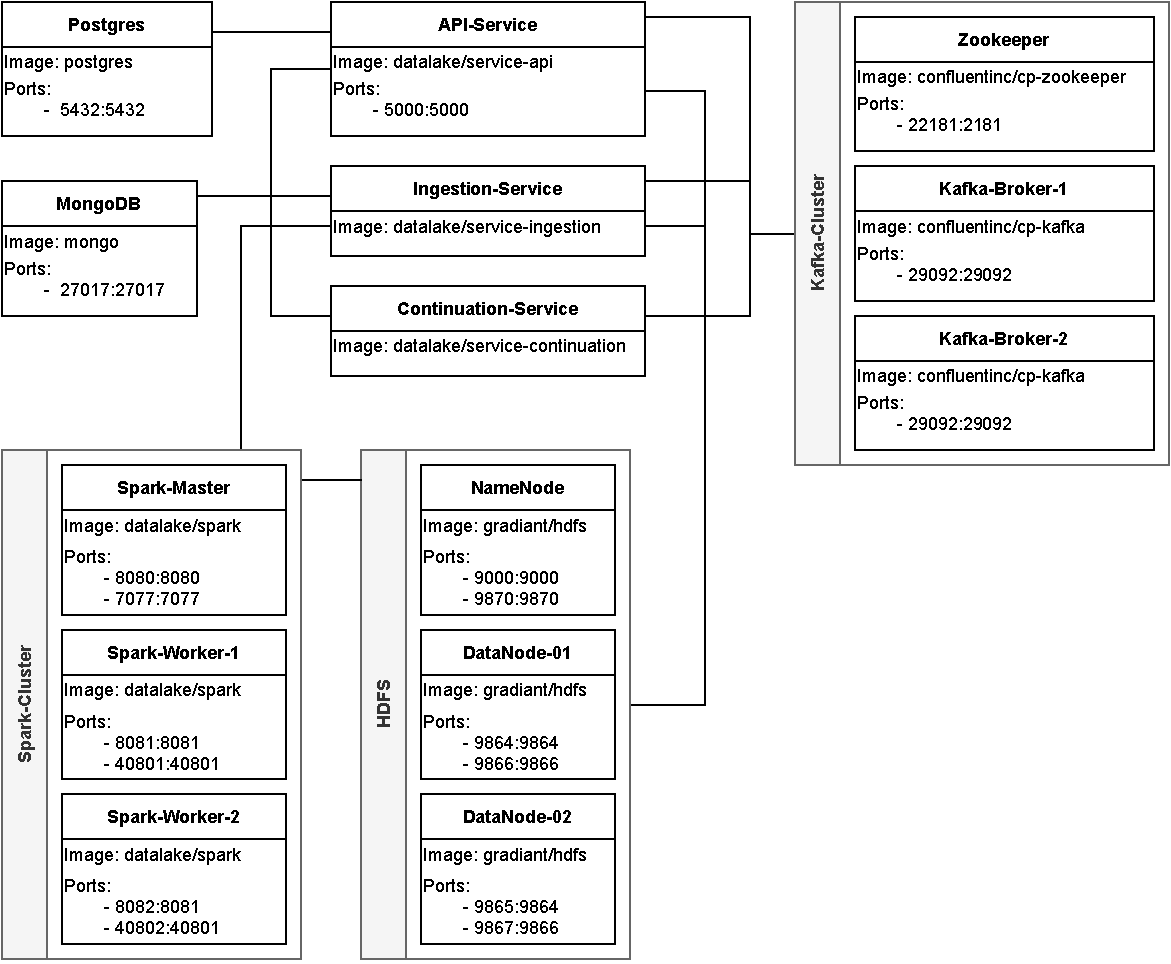
\includegraphics[width=\textwidth]{Grafiken/Umsetzung-Docker-Lake.pdf}
    \caption{Docker-Container für den Data Lake}
    \label{fig:docker-datalake}
\end{figure}
